\documentclass[usenames,dvipsnames]{beamer}
%\documentclass[usenames,dvipsnames,handout]{beamer}

\usetheme{Madrid}
\usecolortheme{dolphin}
\setbeamercolor{title}{fg=NavyBlue}
\setbeamercolor{frametitle}{fg=NavyBlue}
\setbeamercolor{section in toc}{fg=NavyBlue}
\setbeamercolor{block title}{fg=white,bg=NavyBlue}

\usepackage[english]{babel}
\usepackage{amsthm}
\usepackage{graphicx}
\usepackage[utf8x]{inputenc}
\usepackage{mathtools}
\mathtoolsset{showonlyrefs}
\usepackage{appendixnumberbeamer}
%\usepackage{enumitem}
\usepackage{centernot}
\usepackage{tikz}
\usepackage{algorithm}
\usepackage[]{algpseudocode}
\usepackage{caption}
\usetikzlibrary{positioning}
%\setitemize{label=-, leftmargin=*}
\usepackage{booktabs}
\usepackage{natbib}
\usepackage{multicol}
\usepackage[absolute,overlay]{textpos}
\usepackage{eso-pic}

\makeatletter
\def\BState{\State\hskip-\ALG@thistlm}
\makeatother

\usepackage{etoolbox}

\makeatletter
\expandafter\patchcmd\csname\string\algorithmic\endcsname{\itemsep\z@}{\itemsep=1ex plus2pt}{}{}
\makeatother

\DeclarePairedDelimiter{\abs}{\lvert}{\rvert}
\DeclarePairedDelimiter{\norm}{\lVert}{\rVert}
\renewcommand{\Pr}{\mathbb{P}}
\newcommand{\R}{\mathbb{R}}
\newcommand{\Var}{\operatorname{Var}}
\newcommand{\E}{\operatorname{\mathbb{E}}}
\newcommand{\iid}{\ensuremath{\stackrel{\text{iid}}{\sim}}}
\newcommand{\toweak}{\rightharpoonup}
\DeclarePairedDelimiterX{\inprod}[2]{\langle}{\rangle}{#1, #2}
\DeclareMathOperator*{\argmin}{\mathrm{argmin}\;}
\newcommand{\spann}{\mathrm{span}\;}

\newcommand{\SubItem}[1]{
	{\setlength\itemindent{15pt} \item[-] #1}
}

% Theorem blocks
\newenvironment<>{greenblock}[1][]{%
	\setbeamercolor{block title}{fg=white,bg=ForestGreen}%
	\begin{block}#2{#1}}{\end{block}}
\newenvironment<>{redblock}[1][]{%
	\setbeamercolor{block title}{fg=white,bg=red!75!black}%
	\begin{block}#2{#1}}{\end{block}}
\newenvironment<>{orangeblock}[1][]{%
	\setbeamercolor{block title}{fg=white,bg=orange!75!black}%
	\begin{block}#2{#1}}{\end{block}}

% Add numbers and take out navigation symbols
\beamertemplatenavigationsymbolsempty
\setbeamercolor{date in head/foot}{fg=gray, bg=white}
\setbeamercolor{author in head/foot}{fg=white,bg=white}
\setbeamercolor{title in head/foot}{fg=white,bg=white}
\setbeamertemplate{footline}{
	\leavevmode%
	\hbox{%
		\begin{beamercolorbox}[wd=.4\paperwidth,ht=2.25ex,dp=1ex,center]{author in head/foot}%
		\end{beamercolorbox}%
		\begin{beamercolorbox}[wd=.3\paperwidth,ht=2.25ex,dp=1ex,center]{title in head/foot}%
		\end{beamercolorbox}%
		\begin{beamercolorbox}[wd=.3\paperwidth,ht=2.25ex,dp=1ex,right]{date in head/foot}%
			\insertframenumber{} / \inserttotalframenumber\hspace*{2ex} 
	\end{beamercolorbox}}%
	\vskip0pt%
}

\definecolor{leg1}{RGB}{0,114,189}
\definecolor{leg2}{RGB}{217,83,25}
\definecolor{leg3}{RGB}{237,177,32}
\definecolor{leg4}{RGB}{126,47,142}
\definecolor{leg5}{RGB}{119,172,48}

% Text starts always from the top of the frame
\newenvironment{frameT}{\begin{frame}[t]}{\end{frame}}

\title[]{\Large Ensemble Kalman filter for multiscale inverse problems}
%\author[Andrea Zanoni]{Author: Andrea Zanoni \\ Advisors: Professor Assyr Abdulle, Professor Sandro Salsa \\ Co-advisor: Giacomo Garegnani}
\author{Assyr Abdulle, Giacomo Garegnani, Sandro Salsa}
%\date[25/07/2019]{\small Thursday 25 July 2019}
\date{MATHICSE Retreat \\ 11--13 June 2019}
%\date{Place \dots \\ Date \dots}
\institute[Polimi, EPFL]{ 
\begin{multicols}{2}
\centering 
\includegraphics[width=0.1\textwidth]{Images/logo_POLIMI} \\
\columnbreak
\includegraphics[width=0.2\textwidth]{Images/logo_EPFL} \\
\end{multicols}
\vspace{-1cm}
\begin{multicols}{2}
\centering 
POLITECNICO \\ DI MILANO \\
Master in Mathematical \\ Engineering \\
\columnbreak
\'ECOLE POLYTECHNIQUE \\ F\'ED\'ERALE DE LAUSANNE \\
Master in Computational \\ Science and Engineering \\
\end{multicols}
}

\makeatletter
\setbeamertemplate{title page}
{
\vbox{}
\vfill
\begin{centering}
\vspace{-2cm}
{\usebeamercolor[fg]{titlegraphic}\inserttitlegraphic\par}  
\vskip2.25em%
\begin{beamercolorbox}[sep=8pt,center]{institute}
\usebeamerfont{institute}\insertinstitute
\end{beamercolorbox}
\begin{beamercolorbox}[sep=8pt,center]{title}
\usebeamerfont{title}\inserttitle\par%
\ifx\insertsubtitle\@empty%
\else%
\vskip0.25em%
{\usebeamerfont{subtitle}\usebeamercolor[fg]{subtitle}\insertsubtitle\par}%
\fi%    
\end{beamercolorbox}%
\vskip1em\par
\begin{beamercolorbox}[sep=8pt,center]{author}
\usebeamerfont{author}\insertauthor
\end{beamercolorbox}
\vspace{0cm} %<-- right here
\begin{beamercolorbox}[sep=8pt,center]{date}
\usebeamerfont{date}\insertdate
\end{beamercolorbox}\vskip0.5em
\end{centering}
\vfill
}
\makeatother

\newcommand\FrameText[1]{%
	\begin{textblock*}{\paperwidth}(0pt,\textheight)
		\raggedleft #1\hspace{1.5em}
\end{textblock*}}

\begin{document}

\thispagestyle{empty}
\frame{\titlepage}

\begin{frame}
\frametitle{Main ingredients}
\thispagestyle{empty}
\centering
\includegraphics[width=0.9\textwidth]{Images/problem}
\end{frame}

%\addtocounter{framenumber}{-1}

\begin{frame}
\thispagestyle{empty}
\frametitle{Outline}
\tableofcontents
\end{frame}

%\addtocounter{framenumber}{-1}

\section{Inverse problems}

\AtBeginSection[]
{
\begin{frame}<beamer>
\frametitle{Outline}
\thispagestyle{empty}
\tableofcontents[currentsection]
\end{frame}
}

%\begin{frame}
%\frametitle{Inverse problem}
%\begin{equation*}
%\text{find } {\color{ForestGreen} u} \in X \text{ given } {\color{NavyBlue} y} = \mathcal{G}({\color{ForestGreen} u}) + {\color{BrickRed} \eta} \in Y
%\end{equation*}
%where:
%\begin{itemize}
%\item ${\color{ForestGreen} u}$ is the {\color{ForestGreen} unknown}
%\item the parameter space $X$ is a Hilbert space $(X = \mathbb{R}^M)$
%\item ${\color{NavyBlue} y}$ is the {\color{NavyBlue} observation}
%\item the observation space $Y$ is a Hilbert space $(Y = \mathbb{R}^L)$
%\item $\mathcal{G} \colon X \to Y$ is the \textbf{forward operator}
%\item ${\color{BrickRed} \eta}$ is a source of additive {\color{BrickRed} noise}, modelled as a zero mean random variable with covariance operator $\Gamma$
%\end{itemize}
%\end{frame}

\begin{frame}
\frametitle{Inverse problem}
\begin{equation*}
\text{Find } \onslide<2->\underbrace{\onslide<1-> u \in X \onslide<2->}_{\text{unknown}} \onslide<1-> \text{ given } \onslide<2-> \underbrace{\onslide<1-> y = \mathcal{G}(u) + \onslide<2-> \overbrace{\onslide<1-> \eta \onslide<2->}^{\text{noise}}}_{\text{observation}} \onslide<1-> \in Y
\end{equation*}
\vspace{0.5cm}
\onslide<2->
\begin{itemize}
\item $X, Y$ Hilbert spaces
\item $\eta \sim \mathcal{N}(0,\Gamma)$
\vspace{0.5cm}
\onslide<3->
\item $\mathcal{G} \colon X \to Y$ \textbf{forward operator}, $\mathcal{G} = {\color{ForestGreen} \mathcal{O}} \circ {\color{BrickRed} \mathcal{S}}$
\SubItem{${\color{ForestGreen} \mathcal{O}} \colon H^1(\Omega) \to Y$ {\color{ForestGreen} observation operator}}
\SubItem{${\color{BrickRed} \mathcal{S}} \colon X \to H^1(\Omega)$ {\color{BrickRed} solution operator} of PDE}
\begin{equation*}
\begin{cases}
- \nabla \cdot ( A_u \nabla p ) = f & \text{ in } \Omega \\
p = g & \text{ on } \partial \Omega
\end{cases}
\end{equation*}
\end{itemize}
\end{frame}

%\begin{frame}
%\frametitle{Forward operator}
%{\Huge
%\begin{equation*}
%\mathcal{G} = {\color{ForestGreen} \mathcal{O}} \circ {\color{BrickRed} \mathcal{S}}
%\vspace{1cm}
%\end{equation*}}
%where:
%\begin{itemize}
%\item ${\color{ForestGreen} \mathcal{O}} \colon H^1(\Omega) \to Y$ is an {\color{ForestGreen} observation operator}
%\item ${\color{BrickRed} \mathcal{S}} \colon X \to H^1(\Omega)$ is the {\color{BrickRed} solution operator} of a PDE
%\begin{equation*}
%\begin{cases}
%- \nabla \cdot ( A_u \nabla p ) = 0 & \text{ in } \Omega \\
%p = g & \text{ on } \partial \Omega
%\end{cases}
%\end{equation*}
%\end{itemize}
%\end{frame}

\begin{frameT}
\frametitle{Overview of different techniques}
Given a prior $\mu_0$, consider two families of techniques
\vspace{0.5cm}
\begin{itemize}
\item Tikhonov methods $\longrightarrow$ solution is a \textbf{point}
\begin{equation*}
u^* = \argmin_{u \in X} \Big( \underbrace{\Psi(u;y)}_{\text{misfit functional}} + \underbrace{\mathcal{R}(u;\mu_0)}_{\text{regularization term}} \Big)
\end{equation*}
\end{itemize}
%\onslide<2->
\begin{greenblock}[Example]
Least squares with Tikhonov--Phillips regularization ($\mu_0 = \mathcal{N}(\bar{u},C)$)
\begin{equation*}
u^* = u_{\mathrm{TP}} = \argmin_{u \in X} \left ( \norm{y - \mathcal{G}(u)}_{\Gamma}^2 + \norm{u - \bar{u}}_C^2 \right )
\end{equation*}
\end{greenblock}
\end{frameT}

\begin{frameT}
\frametitle{Overview of different techniques}
Given a prior $\mu_0$, consider two families of techniques
\vspace{0.5cm}
\begin{itemize}
\item Bayesian methods $\longrightarrow$ solution is a \textbf{distribution}
\begin{equation*}
\dfrac{d \mu^y}{d \mu_0}(u) \propto \exp \Big(- \underbrace{\Phi(u;y)}_{\text{potential}} \Big)
\end{equation*}
%\onslide<2->
\begin{greenblock}[Example]
Gaussian noise and prior measure ($\eta \sim \mathcal{N}(0,\Gamma)$, $\mu_0 = \mathcal{N}(\bar{u},C)$)
\begin{equation*}
\mu^y(u) \propto \exp \left \{ - \frac{1}{2} \left ( \norm{y - \mathcal{G}(u)}_{\Gamma}^2 + \norm{u - \bar{u}}_C^2 \right ) \right \}
\end{equation*}
\end{greenblock}
\end{itemize}
\end{frameT}

\section{Ensemble Kalman method}

\begin{frame}
\frametitle{Kalman filter}
Kalman filter estimates {\color{ForestGreen} state $z_n$} $\in Z$ of a linear dynamical system
\begin{equation*}
{\color{ForestGreen} z_{n+1}} = G {\color{ForestGreen} z_n}
\end{equation*}
given {\color{NavyBlue} observations $y_n$} $\in Y$
\begin{equation*}
{\color{NavyBlue} y_n} = H {\color{ForestGreen} z_n} + {\color{BrickRed} \eta_n}
\end{equation*}

\vspace{0.25cm}
where
\begin{itemize}
\item $G$ transition matrix
\item $H$ observation matrix
\item ${\color{BrickRed} \eta_n} \sim \mathcal{N}(0,\Gamma)$ {\color{BrickRed} noise}
\end{itemize}
\end{frame}

\begin{frame}
\frametitle{Kalman filter}
\AddToShipoutPictureFG*{
\AtPageUpperLeft{\color{NavyBlue} \put(-20,-40){\makebox[\paperwidth][r]{\shortstack{$z_{n+1} = G z_n$ \\ $y_n = H z_n + \eta_n$}}}}
}
Compute the estimation $\hat{z}_n$ in order to minimize \[ \mathrm{MSE} = \mathbb{E}[(z_n - \hat{z}_n)^T (z_n - \hat{z}_n)] \]
\begin{tikzpicture}[scale=0.75]
\footnotesize
\draw[rounded corners] (0,4) rectangle (3,5.5) node[align=center,pos=.5] {Measurement\\$y_n$};
\draw[] (0,2) rectangle (3,3.5) node[align=center,pos=.5] {Old estimate\\$\hat{z}_{n-1}$};
\draw[->] (3,2.75) -- (4,2.75);
\draw[] (4,2) rectangle (7,3.5) node[align=center,pos=.5] {Prior estimate\\$\hat{z}_n' = G \hat{z}_{n-1}$};
\draw[] (0,0) rectangle (3,1.5) node[align=center,pos=.5] {Old error\\covariance $C_{n-1}$};
\draw[->] (3,0.75) -- (4,0.75);
\draw[] (4,0) rectangle (7,1.5) node[align=center,pos=.5] {Prior error\\covariance $C_n'$};
\draw[->] (7,0.75) -- (8,0.75);
\draw[] (9.5,0.75) ellipse (1.5cm and 0.75cm) node[align=center] {Kalman gain\\$K_n$};
\draw[->] (7,2.75) -- (12,2.75);
\draw[] (12,2) rectangle (15,3.5) node[align=center,pos=.5] {New estimate\\$\hat{z}_n$};
\draw[-] (11,0.75) -- (11.5,0.75);
\draw[-] (11.5,0.75) -- (11.5,4.75);
\draw[-] (3,4.75) -- (11.5,4.75);
\draw[-] (5.5,0) -- (5.5,-0.5);
\draw[-] (9.5,0) -- (9.5,-0.5);
\draw[-] (5.5,-0.5) -- (9.5,-0.5);
\draw[-] (7.5,-0.5) -- (7.5,-1);
\draw[] (12,0) rectangle (15,1.5) node[align=center,pos=.5] {New error\\covariance $C_n$};
\draw[->] (-0.5,0.75) -- (0,0.75);
\draw[->] (-0.5,2.75) -- (0,2.75);
\draw[->] (15,2.75) -- (15.5,2.75);
\draw[-] (7.5,-1) -- (13.75,-1);
\draw[->] (13.75,-1) -- (13.75,0);
\draw[rounded corners] (12,4) rectangle (15,5.5) node[align=center,pos=.5] {Measurement\\$y_{n+1}$};
\draw[->] (15,4.75) -- (15.5,4.75);
\draw[->] (15,0.75) -- (15.5,0.75);
\end{tikzpicture}
\end{frame}

\begin{frame}
\frametitle{Kalman filter for inverse problems}
\begin{greenblock}[Idea (see \cite{EKMFIP})]
Apply Kalman filter to solve inverse problems
\end{greenblock}
\onslide<2->
\begin{redblock}[Issue]
There are no dynamics
\end{redblock}
\onslide<3->
Introduce artificial dynamics
\begin{equation*}
\begin{cases}
z_{n+1} = \Xi(z_n) \\
y_{n} = H z_n + \eta_n
\end{cases}
\end{equation*}
where
\begin{itemize}
\item $z_n = \begin{bmatrix} u_n & v_n \end{bmatrix}^T \in Z = X \times Y$
\item $\Xi(z_n) = \begin{bmatrix} u_n & \mathcal{G}(u_n) \end{bmatrix}^T$, $H = \begin{bmatrix} 0 & I \end{bmatrix}^T$
\end{itemize}
Observations are obtained by randomizing $y$: $y_n = y + \eta_n$
\end{frame}

\begin{frame}
\frametitle{Ensemble Kalman filter}
\begin{itemize}
\item Initial ensemble $z_0$ :  $z_0^{(j)} = \begin{bmatrix} \psi^{(j)} & \mathcal{G}(\psi^{(j)}) \end{bmatrix}^T$, $\psi^{(j)} \sim \mu_0$, $j = 1, \dots, J$
\item Iterate for $n = 1, \dots, N$
\end{itemize}
\vspace{0.1cm}
\begin{tikzpicture}[scale=0.75]
\footnotesize
\draw[rounded corners] (0,4) rectangle (3,5.5) node[align=center,pos=.5] {Measurement\\$y_n^{(j)} = y + \eta_n^{(j)}$};
\draw[] (0,2) rectangle (3,3.5) node[align=center,pos=.5] {Old estimate\\$z_{n-1}^{(j)}$};
\draw[->] (3,2.75) -- (4,2.75);
\draw[] (4,2) rectangle (7,3.5) node[align=center,pos=.5] {Prior estimate\\$\hat{z}_n^{(j)} = \Xi(z_{n-1}^{(j)})$};
\draw[->] (5.5,2) -- (5.5,1.5);
\draw[] (4,0) rectangle (7,1.5) node[align=center,pos=.5] {Sample\\covariance $C_n$};
\draw[->] (7,0.75) -- (8,0.75);
\draw[] (9.5,0.75) ellipse (1.5cm and 0.75cm) node[align=center] {Kalman gain\\$K_n$};
\draw[->] (7,2.75) -- (12,2.75);
\draw[] (12,2) rectangle (15,3.5) node[align=center,pos=.5] {New estimate\\$z_n^{(j)}$};
\draw[-] (11,0.75) -- (11.5,0.75);
\draw[-] (11.5,0.75) -- (11.5,4.75);
\draw[-] (3,4.75) -- (11.5,4.75);
\draw[->] (-0.5,2.75) -- (0,2.75);
\draw[->] (15,2.75) -- (15.5,2.75);
\draw[rounded corners] (12,4) rectangle (15,5.5) node[align=center,pos=.5] {Measurement\\$y_{n+1}^{(j)}$};
\draw[->] (15,4.75) -- (15.5,4.75);
\end{tikzpicture}
\vspace{0.1cm}
 \begin{itemize}
\item Compute the solution $u_{\mathrm{EnKF}} = \frac{1}{J} \sum_{j=1}^J u_{N}^{(j)}$
 \end{itemize}
\end{frame}

%\begin{frame}
%\frametitle{Ensemble Kalman filter algorithm ($\mathrm{EnKF}$)}
%\small
%\begin{algorithmic}[1]
%\State draw {\color{NavyBlue} $J$} samples $\{ \psi^{(j)} \}_{j=1}^J$ from the prior distribution $\mu_0$
%\State construct the initial ensemble $z_0$ as $z_0^{(j)} = \begin{bmatrix} \psi^{(j)} & \mathcal{G}(\psi^{(j)}) \end{bmatrix}^T$
%\For {$n = 0, \dots, {\color{NavyBlue} N}-1$}
%\State propagate the ensemble of particles $\hat{z}_{n+1}^{(j)} = \Xi(z_n^{(j)})$
%\State compute the sample mean $\bar{z}_{n+1} = \frac{1}{J} \sum_{j=1}^J \hat{z}_{n+1}^{(j)}$
%\State compute the sample covariance $C_{n+1} = \frac{1}{J} \sum_{j=1}^J \hat{z}_{n+1}^{(j)} (\hat{z}_{n+1}^{(j)})^T - \bar{z}_{n+1} \bar{z}_{n+1}^T$
%\State define the Kalman gain $K_{n+1} = C_{n+1} H^* (H C_{n+1} H^* + \Gamma)^{-1}$
%\State sample $\eta_{n+1}^{(j)}$ from the distribution $\mathcal{N}(0,\Gamma)$
%\State perturb the data $y_{n+1}^{(j)} = y + \eta_{n+1}^{(j)}$
%\State update the ensemble of particles {\color{BrickRed} $z_{n+1}^{(j)} = \hat{z}_{n+1}^{(j)} + K_{n+1} (y_{n+1}^{(j)} - H \hat{z}_{n+1}^{(j)})$}
%\EndFor
%\State compute the solution {\color{ForestGreen} $u_{\mathrm{EnKF}} = \frac{1}{J} \sum_{j=1}^J H^{\perp} z_{N}^{(j)}$}
%\end{algorithmic}
%\end{frame}

\begin{frame}
\frametitle{Ensemble Kalman filter}
\begin{greenblock}[Properties]
\begin{itemize}
\item $u_{\mathrm{EnKF}} \in \spann \left ( \{ \psi^{(j)} \}_{j=1}^J \right )$ 
\item If $\mathcal{G}$ \textbf{linear} then $u_{\mathrm{EnKF}}(N=1) \to u_{\mathrm{TP}} \text{ as } J \to \infty$
\item Easily parallelizable
\end{itemize}
\end{greenblock}
\vspace{1cm}
\onslide<2->
\begin{orangeblock}[Warning]
$J \cdot N$ evaluations of the forward operator $\mathcal{G}$ required
\end{orangeblock}
\end{frame}

\section{Multiscale inverse problems}

\begin{frame}
\frametitle{Multiscale inverse problems}
\begin{equation*}
\text{Find } {\color{ForestGreen} u} \in X \text{ given } {\color{NavyBlue} y} = \mathcal{G}^{\varepsilon}({\color{ForestGreen} u}) + {\color{BrickRed} \eta} \in Y
\end{equation*}
where
\begin{equation*}
\mathcal{G}^{\varepsilon} = \mathcal{O} \circ \mathcal{S}^{\varepsilon}
\end{equation*}
and $\mathcal{S}^{\varepsilon}$ is the solution operator of a multiscale PDE
\begin{minipage}[t]{0.59\textwidth}
\begin{equation*}
\begin{cases}
- \nabla \cdot ( A_{u}^{\varepsilon} \nabla p^{\varepsilon} ) = f & \text{ in } \Omega \\
p^{\varepsilon} = g & \text{ on } \partial \Omega
\end{cases}
\end{equation*}
\end{minipage}
\begin{minipage}[t]{0.39\textwidth}
\[ A_u^{\varepsilon}(x) = A \left ( u(x), \frac{x}{\varepsilon} \right ) \]
\end{minipage}

\vspace{0.5cm}
\onslide<2->
\begin{redblock}[Issue]
Evaluation of $\mathcal{G}^{\varepsilon}$ computationally very expensive if $\varepsilon \ll 1$
\end{redblock}
\end{frame}

\begin{frame}
\frametitle{Homogenization}
\begin{theorem}%[see \cite{IH}]
There exist $A^0_u$ and $p^0$ such that 
\[ p^{\varepsilon} \toweak p^0 \text{ in } H^1(\Omega) \]
where $p^0$ is the solution of
\begin{equation*}
\begin{cases}
- \nabla \cdot (A_u^0 \nabla p^0) = f & \text{ in } \Omega \\
p^0 = g & \text{ on } \partial \Omega
\end{cases}
\end{equation*}
\end{theorem}
\onslide<2->
\begin{greenblock}[Idea (see \cite{MMIP})]
Replace $\mathcal{G}^{\varepsilon}$ with $\mathcal{G}^0_h = \mathcal{O} \circ \mathcal{S}^0_h$, where $\mathcal{S}^0_h$ is the solution operator corresponding to the FEM discretizazion of the homogenized problem
\end{greenblock}
\end{frame}

\begin{frame}
\frametitle{A one-dimensional example}
\begin{figure}
\hspace{0.65cm}
\includegraphics[scale=0.8]{Images/legend_p}
\hspace{1.85cm}
\includegraphics[scale=0.8]{Images/legend_sigma_a}
\\	
\includegraphics[width=0.35\textwidth]{Images/p_09}
\hspace{1cm}
\includegraphics[width=0.35\textwidth]{Images/sigma_homogenized_09}
\\
\includegraphics[width=0.35\textwidth]{Images/p_01}
\hspace{1cm}
\includegraphics[width=0.35\textwidth]{Images/sigma_homogenized_01}
\caption{Left: solution of the PDE. Right: unknown of the inverse problem.}
\end{figure}
\end{frame}

\begin{frame}
\frametitle{Convergence analysis}
\begin{itemize}
\item $u_N^{\varepsilon} = \{ u_N^{\varepsilon(j)} \}_{j=1}^J$ ensemble generated by $\mathrm{EnKF}$ with $\mathcal{G}^{\varepsilon}$
\item $u^0_{N,h} = \{ u^{0(j)}_{N,h} \}_{j=1}^J$ ensemble generated by $\mathrm{EnKF}$ with $\mathcal{G}^0_h$
\item norm of the ensemble defined by
\[ \norm{u} \vcentcolon = \frac{1}{J} \sum_{j=1}^J \norm{u^{(j)}}_X \]
\end{itemize}
\onslide<2->
\begin{greenblock}[Main assumptions]
\begin{itemize}
%\item $\norm{\mathcal{O}(p_1) - \mathcal{O}(p_2)}_2 \le m \norm{p_1 - p_2}_{L^2(\Omega)}$
%\item $u_n^{(j)} \in B_R(u^*) \text{ for all } j = 1, \dots, J \text{ and } n = 1, \dots, N$
%\item $\norm{A(u_1) - A(u_2)}_{L^{\infty}(\Omega;\R^{N \times N})} \le M \norm{u_1 - u_2}_2$
%\item $A(u) \xi \cdot \xi \ge \alpha \norm{\xi}_2^2$
\item $\mathcal{O}$ Lipschitz from $L^2$ to $Y$
\item $A$ elliptic and Lipschitz from $X$ to $L^{\infty}$
\item Algorithm stable
\end{itemize}
\end{greenblock}
\end{frame}

\begin{frame}
\frametitle{Convergence analysis}
\begin{theorem}
Under the previous assumptions
\begin{equation*}
\mathbb{E} \left [ \norm{u_N^{\varepsilon} - u_{N,h}^0} \right ] \le C ( \varepsilon + h^{s+1} )
\end{equation*}
where $s = \min \{ r, q \}$, $p^0 \in H^{q+1}(\Omega)$ and $r$ degree of the FEM basis
%\begin{itemize}
%\item $p^0 \in H^{q+1}(\Omega)$
%\item $r$ is the degree of the FEM basis
%\end{itemize}
%In particular
%\begin{equation*}
%\mathbb{E} \left [ \norm{u_N^{\varepsilon} - u_{N,h}^0} \right ] \to 0 \qquad \text{as} \qquad \varepsilon, h \to 0
%\end{equation*}
\end{theorem}
\onslide<2->
\textbf{Idea of the proof}
\begin{itemize}
\item Let $u_N^0 = \{ u_N^{0(j)} \}_{j=1}^J$ be the ensemble generated by $\mathrm{EnKF}$ with $\mathcal{G}^0$
\item By triangle inequality
\begin{equation*}
\mathbb{E} \left [ \norm{u_N^{\varepsilon} - u_{N,h}^0} \right ] \le \underbrace{\mathbb{E} \left [ \norm{u_N^{\varepsilon} - u_N^0} \right ]}_{\let\scriptstyle\textstyle \substack{\text{\small multiscale} \\ \text{\small convergence} \\ \varepsilon \to 0 \vspace{0.1cm} \\ \Downarrow \vspace{0.1cm} \\ \le C_1 \varepsilon}} + \underbrace{\mathbb{E} \left [ \norm{u_N^0 - u_{N,h}^0} \right ]}_{\let\scriptstyle\textstyle \substack{\text{\small FEM} \\ \text{\small convergence} \\ h \to 0 \vspace{0.1cm} \\ \Downarrow \vspace{0.1cm} \\ \le C_2 h^{s+1}}}
\end{equation*}
\end{itemize}
\end{frame}

%\begin{frame}
%\frametitle{Convergence analysis}
%\textbf{Idea of the proof}
%\vspace{0.5cm}
%\begin{itemize}
%\item Let $u_N^0 = \{ u_N^{0(j)} \}_{j=1}^J$ be the ensemble generated by $\mathrm{EnKF}$ with $\mathcal{G}^0$
%\vspace{0.5cm}
%\item By triangle inequality
%\begin{equation*}
%\mathbb{E} \left [ \norm{u_N^{\varepsilon} - u_{N,h}^0} \right ] \le \underbrace{\mathbb{E} \left [ \norm{u_N^{\varepsilon} - u_N^0} \right ]}_{\let\scriptstyle\textstyle \substack{\text{\small multiscale} \\ \text{\small convergence} \\ \varepsilon \to 0 \vspace{0.25cm} \\ \Big\Downarrow \vspace{0.25cm} \\ \le C_1 \varepsilon}} + \underbrace{\mathbb{E} \left [ \norm{u_N^0 - u_{N,h}^0} \right ]}_{\let\scriptstyle\textstyle \substack{\text{\small FEM} \\ \text{\small convergence} \\ h \to 0 \vspace{0.25cm} \\ \Big\Downarrow \vspace{0.25cm} \\ \le C_2 h^{s+1}}}
%\end{equation*}
%%\item $\mathbb{E} \left [ \norm{u_N^{\varepsilon} - u_N^0} \right ] \le \sum_{n=0}^{N-1} K_{1,n} \mathbb{E} \left [ \frac{1}{J} \sum_{j=1}^J \underbrace{\norm{\mathcal{S}^{\varepsilon}(u_n^{0(j)}) - \mathcal{S}^0(u_n^{0(j)})}_2}_{\textstyle \le C_1 \varepsilon} \right ]$
%%\item $\mathbb{E} \left [ \norm{u_N^0 - u_{N,h}^0} \right ] \le \sum_{n=0}^{N-1} K_{2,n} \mathbb{E} \left [ \frac{1}{J} \sum_{j=1}^J \underbrace{\norm{\mathcal{S}^0(u_n^{0(j)}) - \mathcal{S}^0_h(u_n^{0(j)})}_2}_{\textstyle \le C_2 h^{s+1}} \right ]$
%\end{itemize}
%\end{frame}

\begin{frame}
\frametitle{Bayesian interpretation of the ensemble Kalman filter}
Posterior distribution approximated by sum of Dirac masses (see \cite{AEKFIP})
\[ \mu_N = \frac{1}{J} \sum_{j=1}^J \delta_{u_N^{(j)}} \]
\begin{itemize}
\item $\mu_N^{\varepsilon} = \frac{1}{J} \sum_{j=1}^J \delta_{u_N^{\varepsilon(j)}}$ posterior generated by $\mathrm{EnKF}$ with $\mathcal{G}^{\varepsilon}$
\item $\mu^0_{N,h} = \frac{1}{J} \sum_{j=1}^J \delta_{u_{N,h}^{0(j)}}$ posterior generated by $\mathrm{EnKF}$ with $\mathcal{G}^0_h$
\end{itemize}
\onslide<2->
\begin{orangeblock}[Warning]
The posterior distributions are random probability measures 
\end{orangeblock}
\end{frame}

\begin{frame}
\frametitle{Convergence of the posterior distributions}
\begin{theorem}
Under the same assumptions of the convergence result
\begin{equation*}
\mu_N^{\varepsilon} - \mu_{N,h}^0 \xrightharpoonup{L^1} 0 \qquad \text{as} \qquad \varepsilon, h \to 0
\end{equation*}
which means
\begin{equation*}
\mathbb{E} \left [ \left | \int f \; \mathrm{d} \mu_N^{\varepsilon} - \int f \; \mathrm{d} \mu_{N,h}^0 \right | \right ] \to 0
\end{equation*}
for all bounded and continuous functions $f \in C^0_B$
\end{theorem}
\onslide<2->
\textbf{Idea of the proof} \\
\begin{itemize}
\item Exploit properties of Wasserstein distance to quantify distance between discrete measures
\item Apply convergence result presented before
\end{itemize}
\end{frame}

%\begin{frame}
%\frametitle{Idea of the proof}
%\begin{itemize}
%\item Show that 
%\begin{equation*}
%\mathbb{E}[W_{1,2}(\mu_N^{\varepsilon}, \mu_{N,h}^0)] \le \mathbb{E}[\norm{u_N^{\varepsilon} - u_{N,h}^0}] \to 0
%\end{equation*}
%where $W_{1,2}$ is the Wasserstein distance
%\begin{equation*}
%W_{1,2}(\mu_N^{\varepsilon}, \mu_{N,h}^0) = \inf_{\gamma \in \Gamma(\mu_N^{\varepsilon}, \mu_{N,h}^0)} \int_{B_R(u^*) \times B_R(u^*)} \norm{v - w}_2 d \gamma(v,w)
%\end{equation*}
%and $\Gamma(\mu_N^{\varepsilon}, \mu_{N,h}^0)$ denotes the collection of all joint distributions on $B_R(u^*) \times B_R(u^*)$ with marginals $\mu_N^{\varepsilon}$ and $\mu_{N,h}^0$
%\item Show that if
%\begin{equation*}
%\mathbb{E}[W_{1,2}(\mu_N^{\varepsilon}, \mu_{N,h}^0)] \to 0
%\end{equation*}
%then
%\begin{equation*}
%\mu_N^{\varepsilon} - \mu_{N,h}^0 \xrightharpoonup{L^1} 0
%\end{equation*}
%\end{itemize}
%\end{frame}

\section{Numerical experiments}

\begin{frame}
\frametitle{Observations and exact solution}
Setting from \cite{BNHMEMIP}
\begin{minipage}{0.44\textwidth}
\centering
Measurements $(i = 1, \dots, 12)$
\begin{equation*}
y_i = \int_{\Gamma_i} A^{\varepsilon} \nabla p_k^{\varepsilon} \cdot \nu \phi_i ds + \eta_i
\end{equation*}
%The measurements are the integrals of the normal flux multiplied by hat functions with compact support in some portions of the boundary
\end{minipage}
\begin{minipage}{0.54\textwidth}
\centering
\begin{tikzpicture}[scale = 0.3]
\draw[-] (0,0) -- (0,10);
\draw[-] (0,10) -- (10,10);
\draw[-] (10,10) -- (10,0);
\draw[-] (10,0) -- (0,0);
\draw[line width = 1mm, NavyBlue] (0,1) -- (0,3);
\draw[line width = 1mm, NavyBlue] (0,4) -- (0,6);
\draw[line width = 1mm, NavyBlue] (0,7) -- (0,9);
\draw[line width = 1mm, NavyBlue] (1,0) -- (3,0);
\draw[line width = 1mm, NavyBlue] (4,0) -- (6,0);
\draw[line width = 1mm, NavyBlue] (7,0) -- (9,0);
\draw[line width = 1mm, NavyBlue] (10,1) -- (10,3);
\draw[line width = 1mm, NavyBlue] (10,4) -- (10,6);
\draw[line width = 1mm, NavyBlue] (10,7) -- (10,9);
\draw[line width = 1mm, NavyBlue] (1,10) -- (3,10);
\draw[line width = 1mm, NavyBlue] (4,10) -- (6,10);
\draw[line width = 1mm, NavyBlue] (7,10) -- (9,10);
\end{tikzpicture}
\vspace{0.5cm}
\end{minipage}
\begin{minipage}{0.44\textwidth}
\centering
Exact unknown
%The exact unknown, which has to be estimated, is
\end{minipage}
\begin{minipage}{0.54\textwidth}
\centering
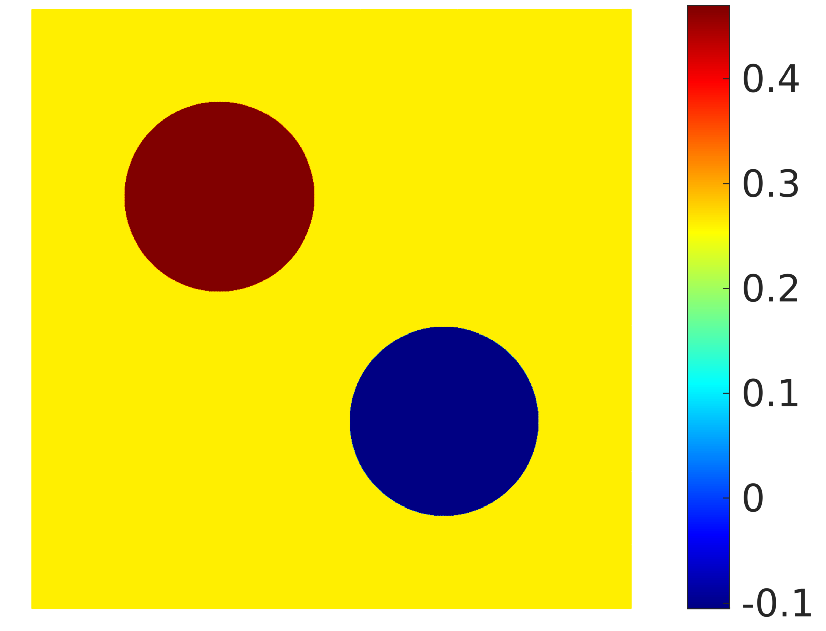
\includegraphics[width=0.7\textwidth]{Images/sigma_exact}
\end{minipage}
\end{frame}

\begin{frame}
\frametitle{Sensitivity w.r.t. $N$}
\begin{figure}[t]
\centering
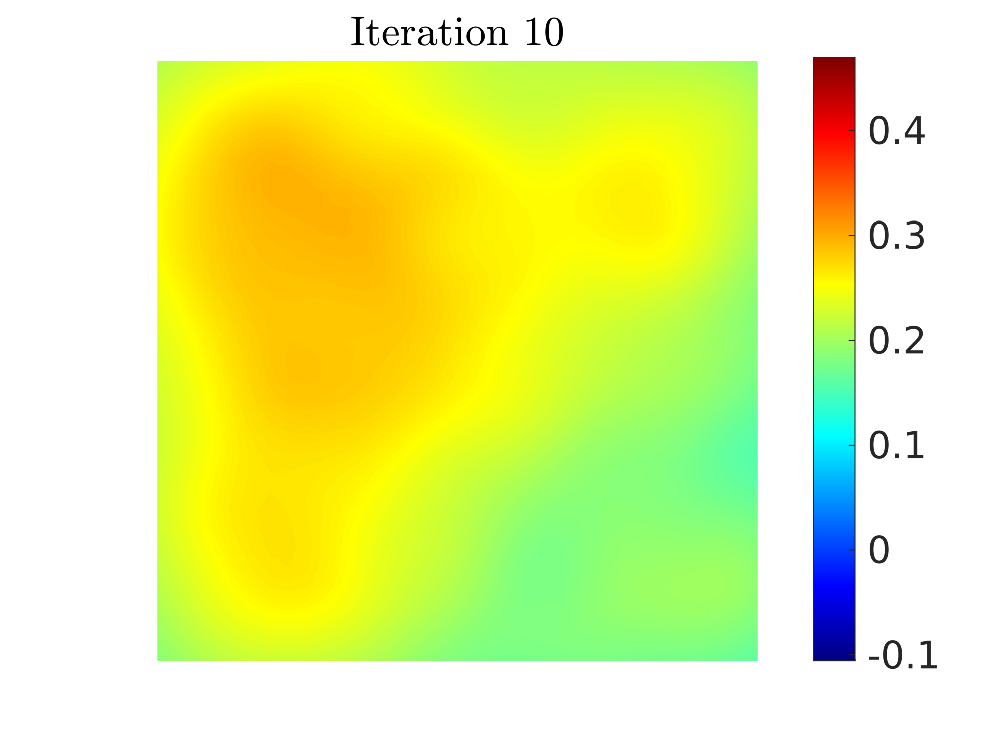
\includegraphics[width = 0.45\textwidth]{Images/ensemble_10}
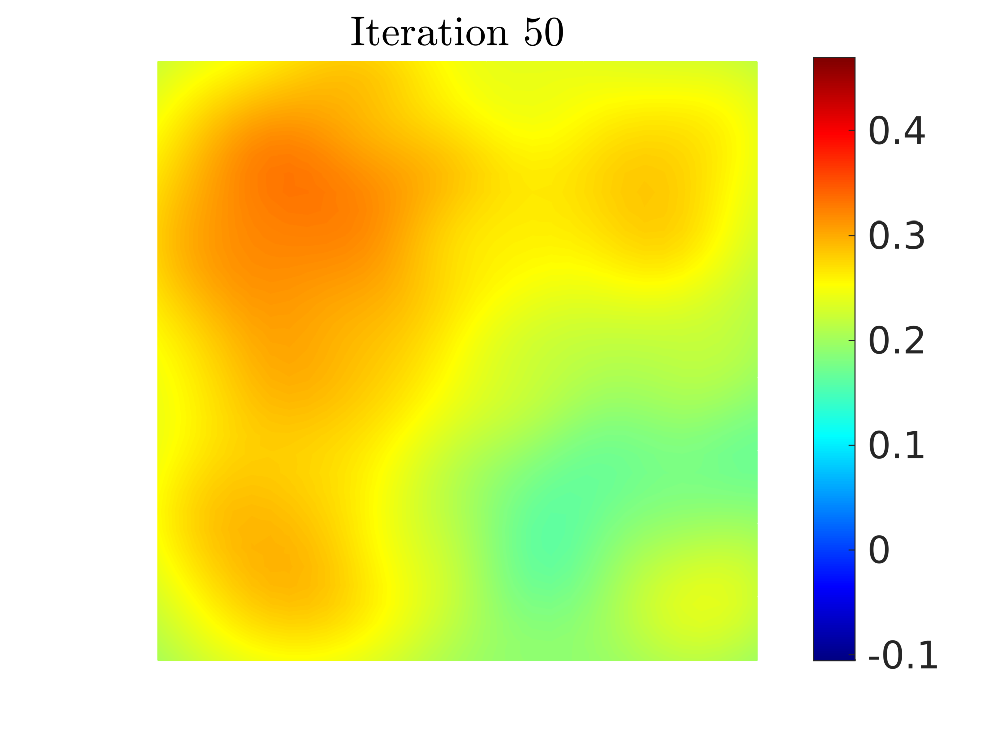
\includegraphics[width = 0.45\textwidth]{Images/ensemble_50}
\\
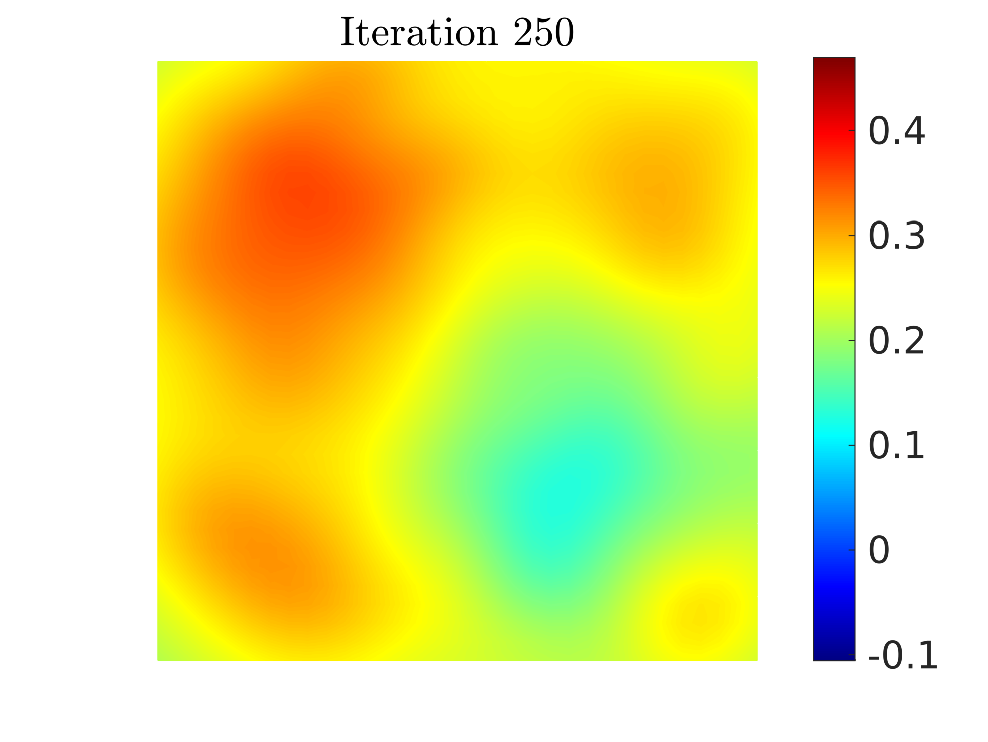
\includegraphics[width = 0.45\textwidth]{Images/ensemble_250}
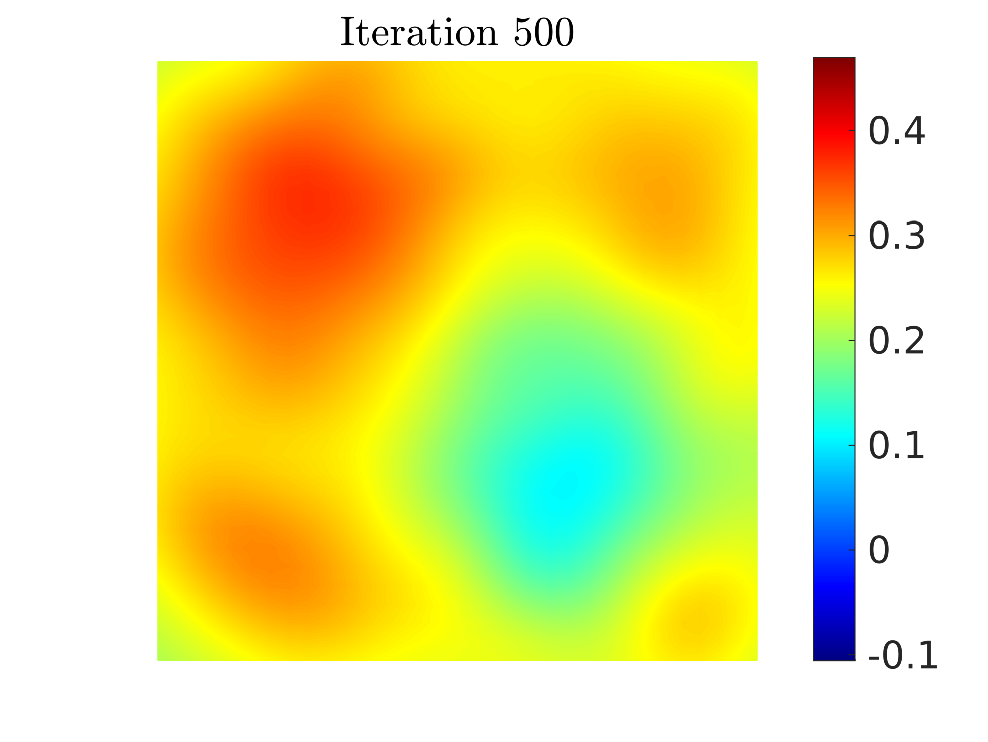
\includegraphics[width = 0.45\textwidth]{Images/ensemble_500}
\end{figure}
\end{frame}

\begin{frame}
\frametitle{Sensitivity w.r.t. $J$}
\begin{figure}[t]
\centering
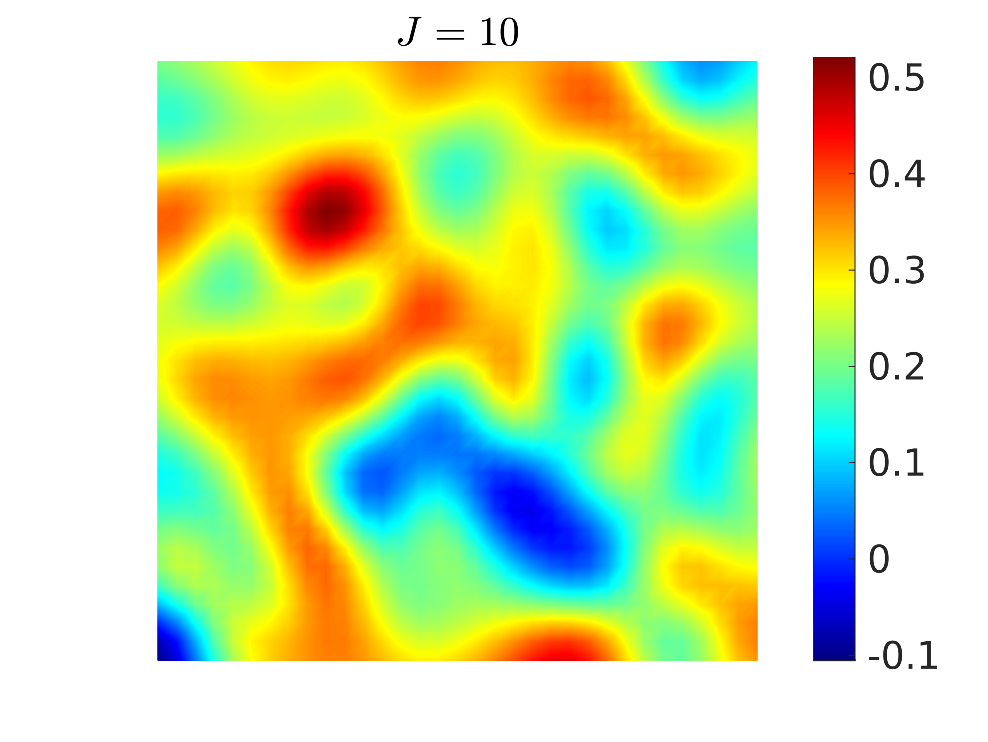
\includegraphics[width = 0.45\textwidth]{Images/ensemble_500_J10}
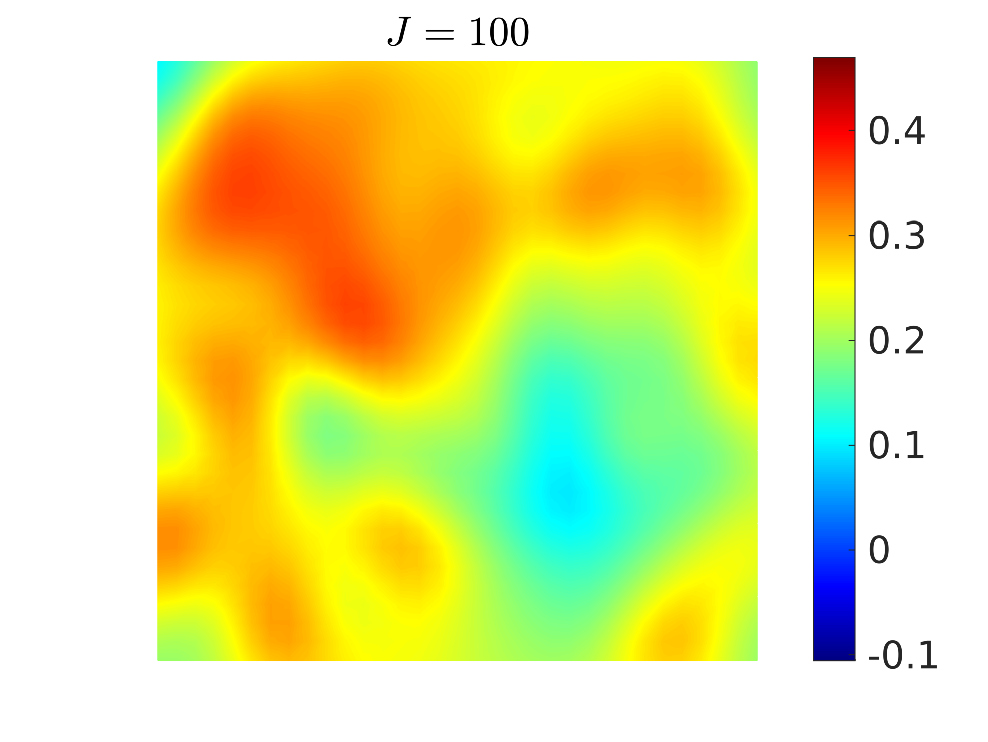
\includegraphics[width = 0.45\textwidth]{Images/ensemble_500_J100}
\\
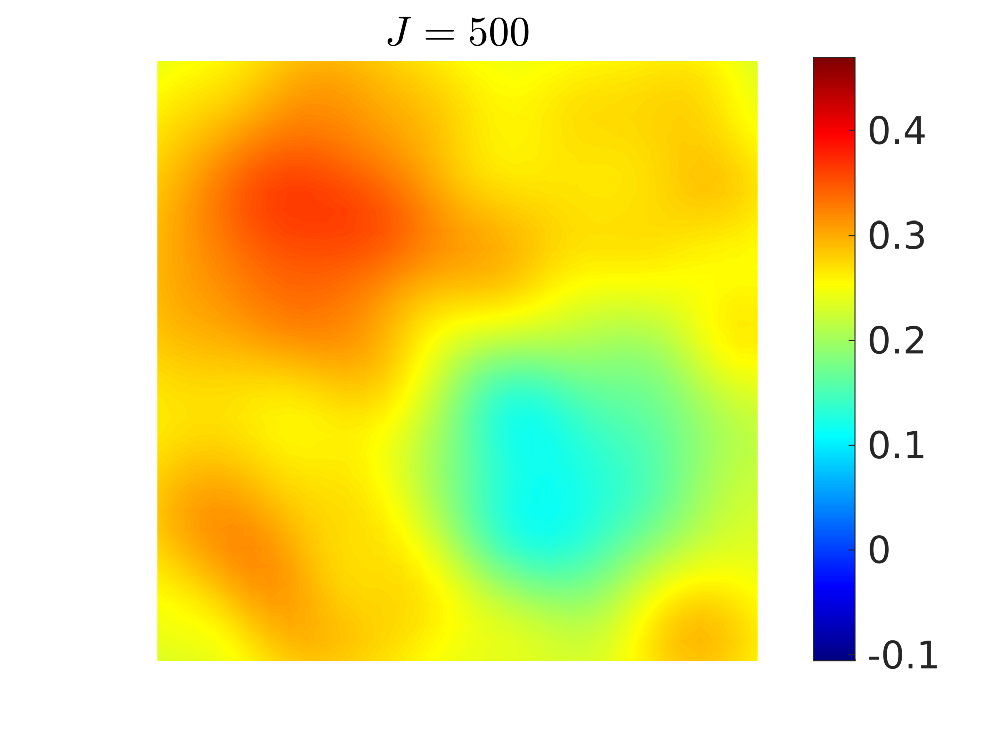
\includegraphics[width = 0.45\textwidth]{Images/ensemble_500_J500}
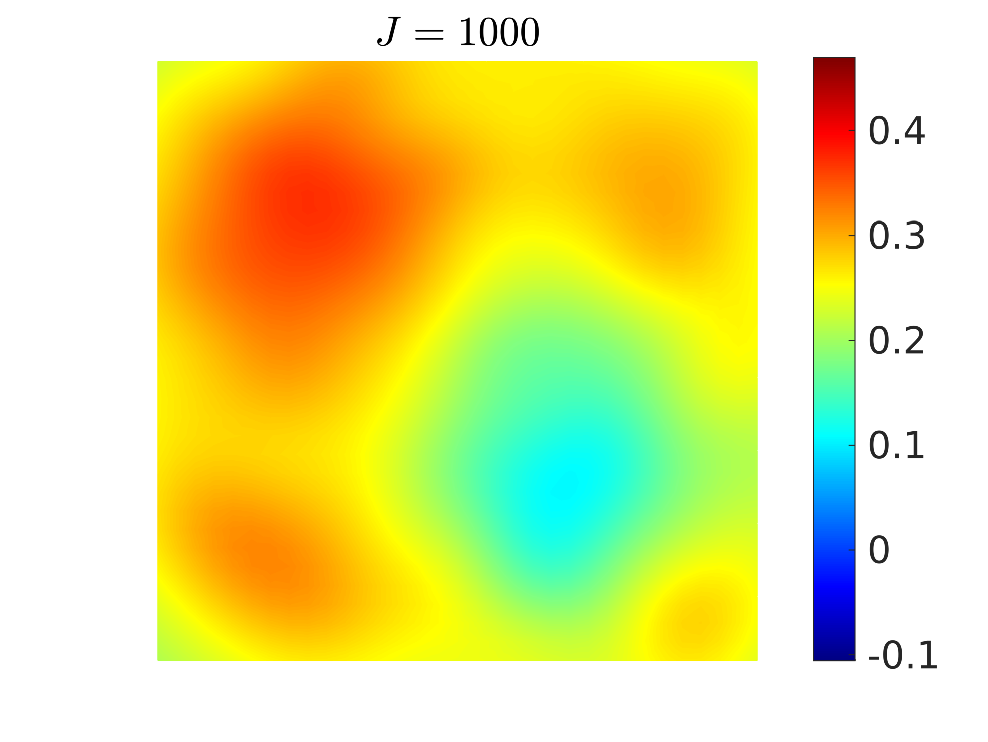
\includegraphics[width = 0.45\textwidth]{Images/ensemble_500_J1000}
\end{figure}
\end{frame}

\begin{frame}
\frametitle{Sensitivity w.r.t. $\varepsilon$}
\begin{figure}[t]
\centering
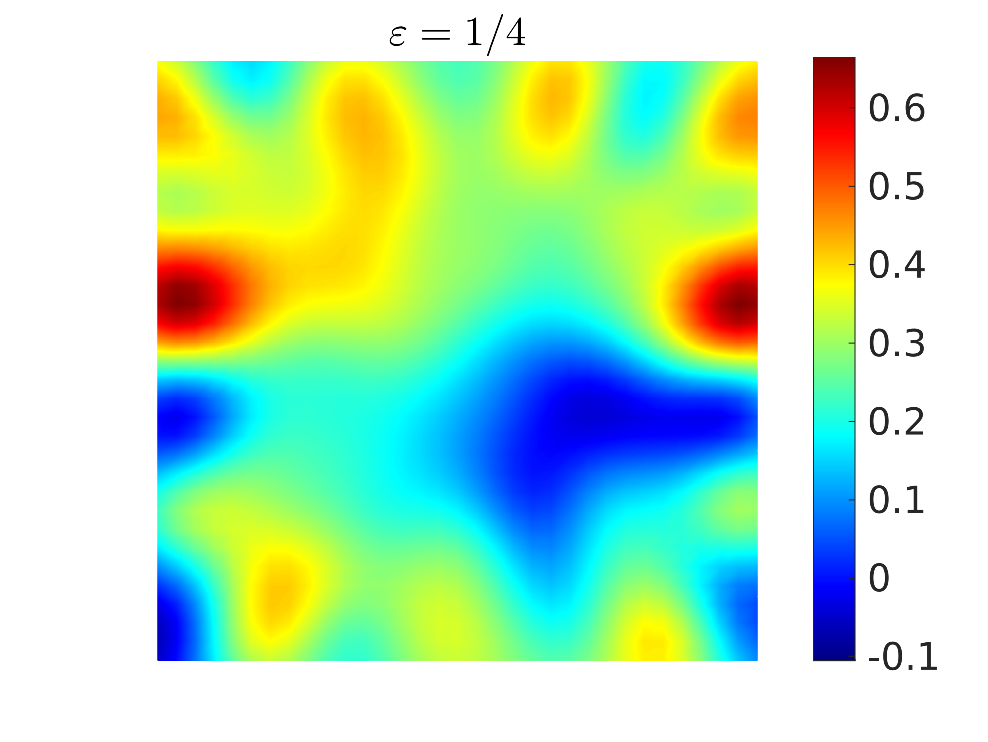
\includegraphics[width = 0.45\textwidth]{Images/ensemble_500_e4}
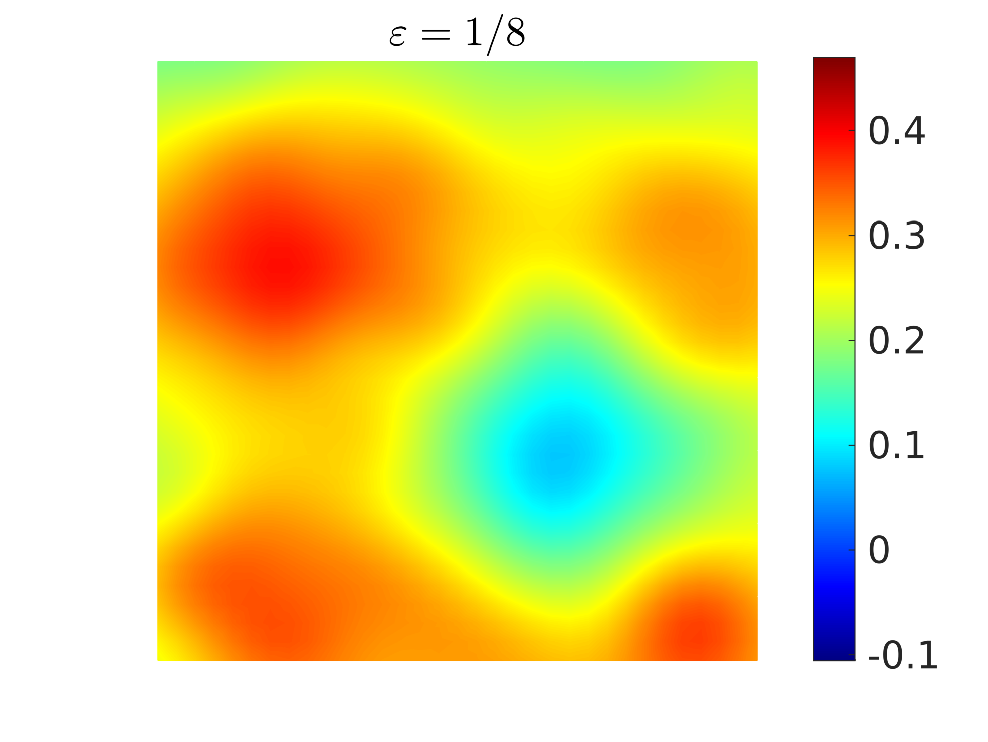
\includegraphics[width = 0.45\textwidth]{Images/ensemble_500_e8}
\\
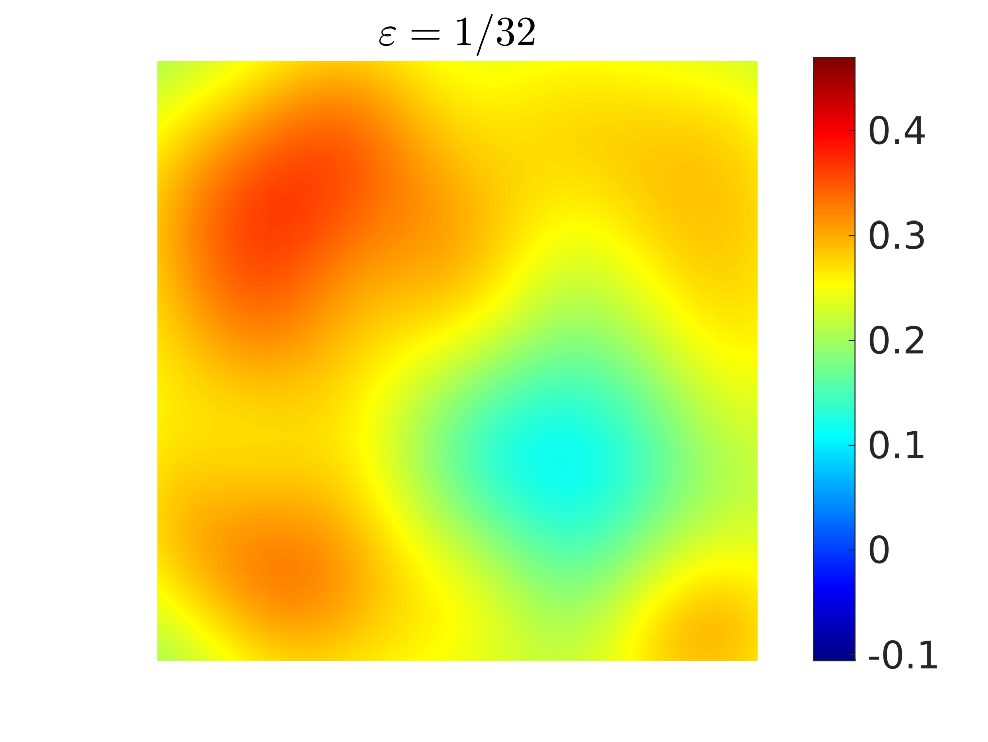
\includegraphics[width = 0.45\textwidth]{Images/ensemble_500_e32}
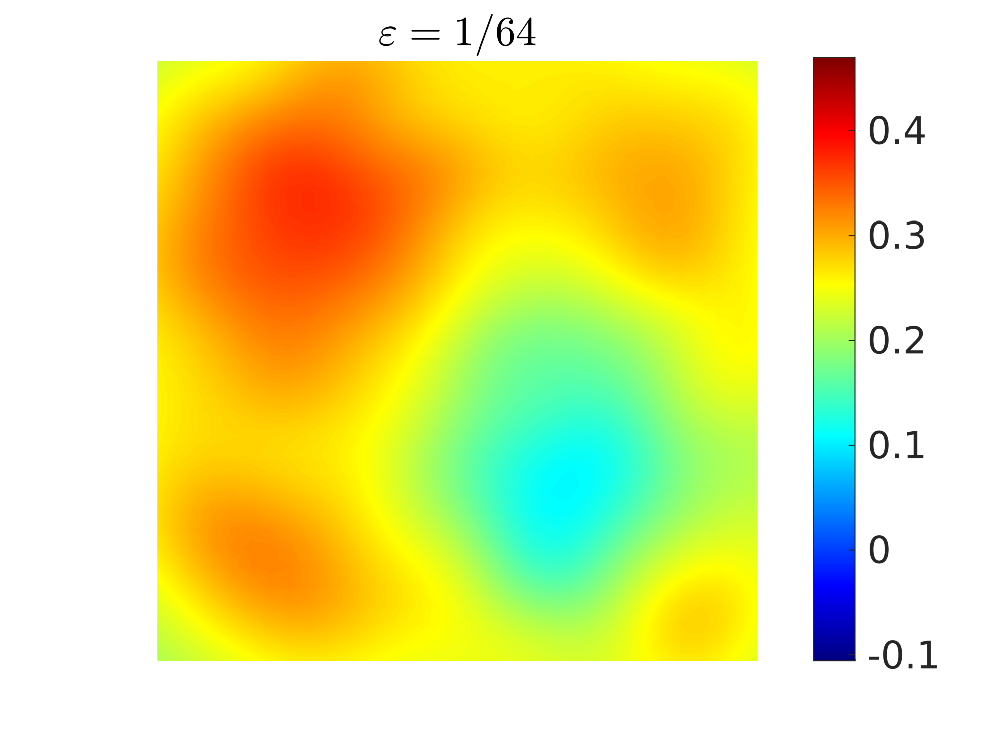
\includegraphics[width = 0.45\textwidth]{Images/ensemble_500_e64}
\end{figure}
\end{frame}

\begin{frame}
\frametitle{Modelling error}
\begin{greenblock}[Idea (see \cite{SCIP})]
The observation can be seen as data generated by the discrete homogenized operator affected by two sources of error 
\begin{equation*}
y = \mathcal{G}^0_h(u^*) + \underbrace{[ \mathcal{G}^{\varepsilon}(u^*) - \mathcal{G}^0_h(u^*) ]}_{\textstyle = \;  \mathcal{E}} + \eta
\end{equation*}
\end{greenblock}

\vspace{0.5cm}
\onslide<2->
Assume that
\[ \mathcal{E} \sim \mathcal{N}(m,\Sigma) \]
then $\mathcal{E} = m + \zeta$ with $\zeta \sim \mathcal{N}(0,\Sigma)$ and
\begin{equation*}
\underbrace{y - m}_{\textstyle = \; \tilde{y}} = \mathcal{G}^0_h(u^*) + \underbrace{\zeta + \eta}_{\textstyle = \; \tilde{\eta}}
\end{equation*}
\end{frame}

\begin{frame}
\frametitle{Estimation of the sample mean $m$ and covariance $\Sigma$}
Two approaches can be followed
\begin{enumerate}%[label=\bullet]
\item<1-> \textbf{offline:} 
\begin{itemize}
\item{sample $\{ u_i \}_{i=1}^{N_{\mathcal{E}}}$ from the prior distribution $\mu_0$}
\item{compute $\mathcal{E}_i = \mathcal{G}^{\varepsilon}(u_i) - \mathcal{G}^0_h(u_i)$}
\item{$m = \frac{1}{N_{\mathcal{E}}} \sum_{i=1}^{N_{\mathcal{E}}} \mathcal{E}_i$ and $\Sigma = \frac{1}{N_{\mathcal{E}}} \sum_{i=1}^{N_{\mathcal{E}}} (\mathcal{E}_i - m) (\mathcal{E}_i - m)^T$}
\end{itemize}
\item<2-> \textbf{online:} subdivide the $\mathrm{EnKF}$ in $\mathcal{L}$ levels, each one with $N^{\ell}$ iterations
\begin{itemize}
\item{sample $\{ u_i^{\ell} \}_{i=1}^{N^{\ell}_{\mathcal{E}}}$ from the distribution $\mu_0^{\ell}$ ($\mu_0^{\ell+1} = \mu_{N^{\ell}}^{\ell}$)}
\item{compute $\mathcal{E}_i^{\ell} = \mathcal{G}^{\varepsilon}(u_i^{\ell}) - \mathcal{G}^0_h(u_i^{\ell})$}
\item{$m^{\ell} = \frac{1}{N_{\mathcal{E}}^{\ell}} \sum_{i=1}^{N_{\mathcal{E}}^{\ell}} \mathcal{E}_i^{\ell}$ and $\Sigma^{\ell} = \frac{1}{N_{\mathcal{E}}^{\ell}} \sum_{i=1}^{N_{\mathcal{E}}^{\ell}} (\mathcal{E}_i^{\ell} - m^{\ell}) (\mathcal{E}_i^{\ell} - m^{\ell})^T$}
\end{itemize}
\end{enumerate}
\onslide<3->
\begin{orangeblock}[Warning]
Online approximation is better, but computationally more expensive
\end{orangeblock}
\end{frame}

\begin{frame}
\frametitle{Offline modelling error estimation}
\begin{figure}[t]
\centering
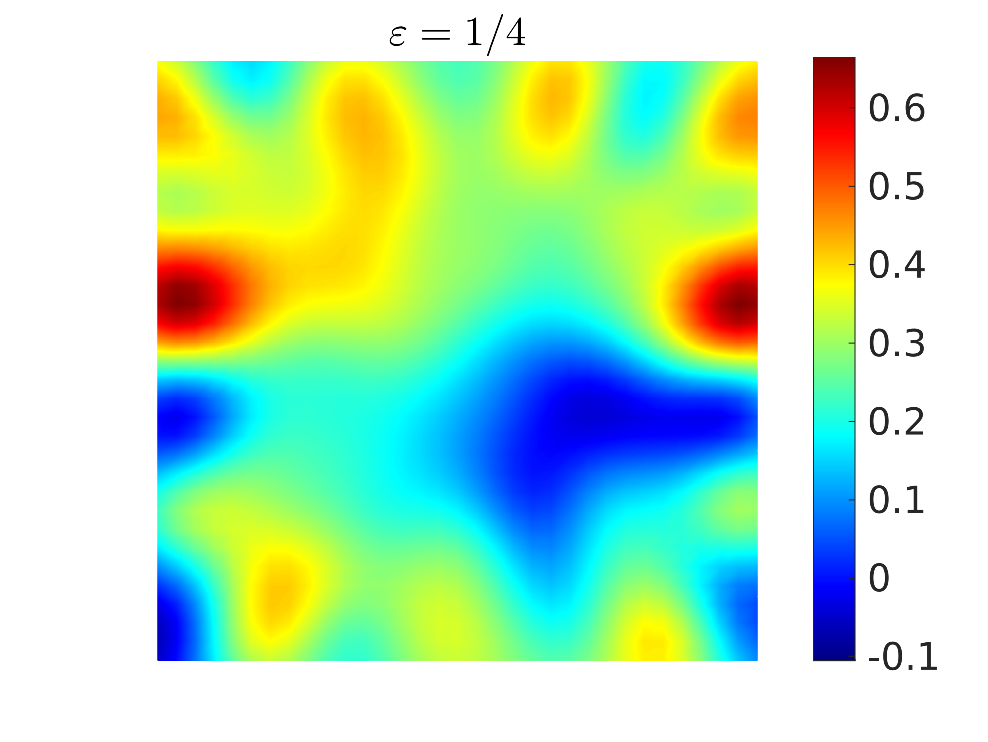
\includegraphics[width = 0.45\textwidth]{Images/ensemble_500_e4}
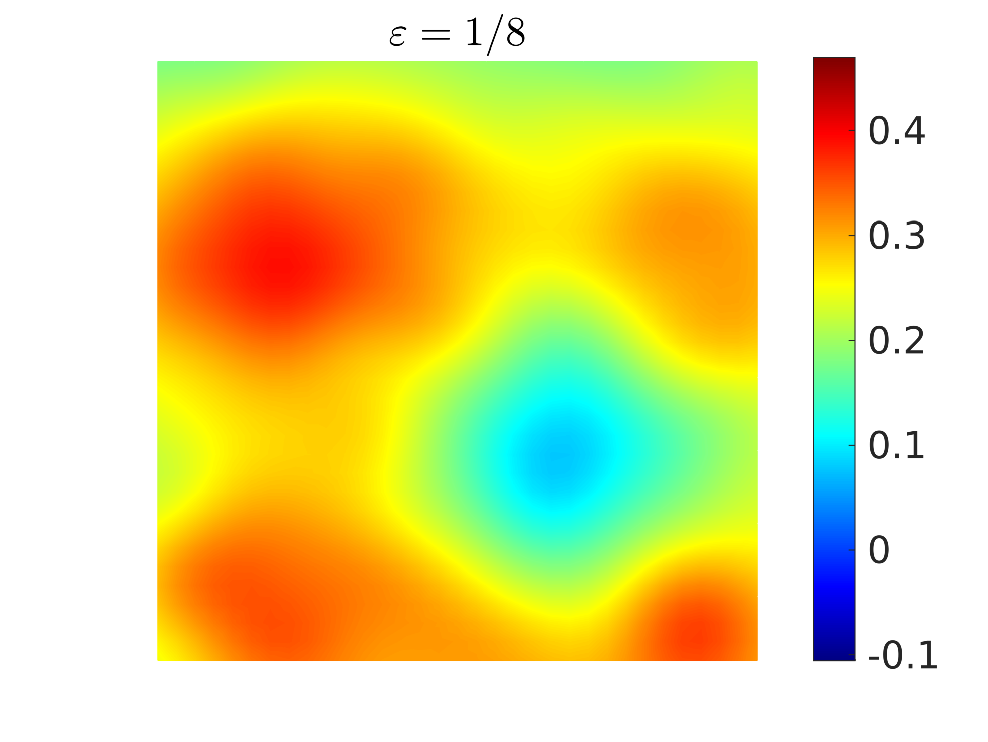
\includegraphics[width = 0.45\textwidth]{Images/ensemble_500_e8}
\\
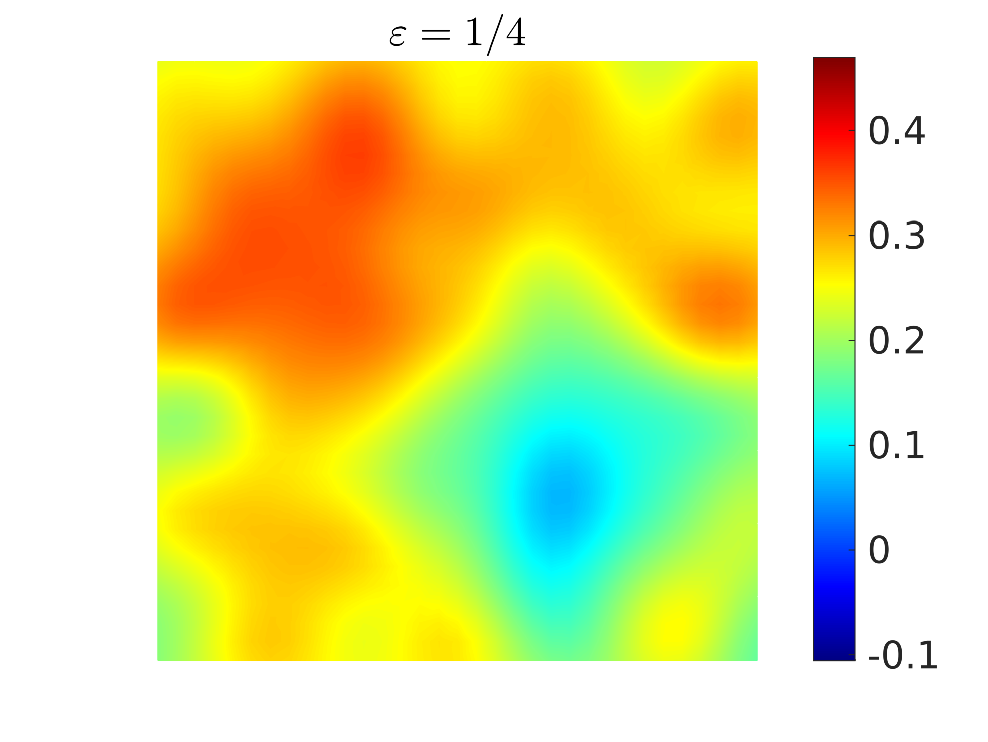
\includegraphics[width = 0.45\textwidth]{Images/ensemble_500_e4_model_error}
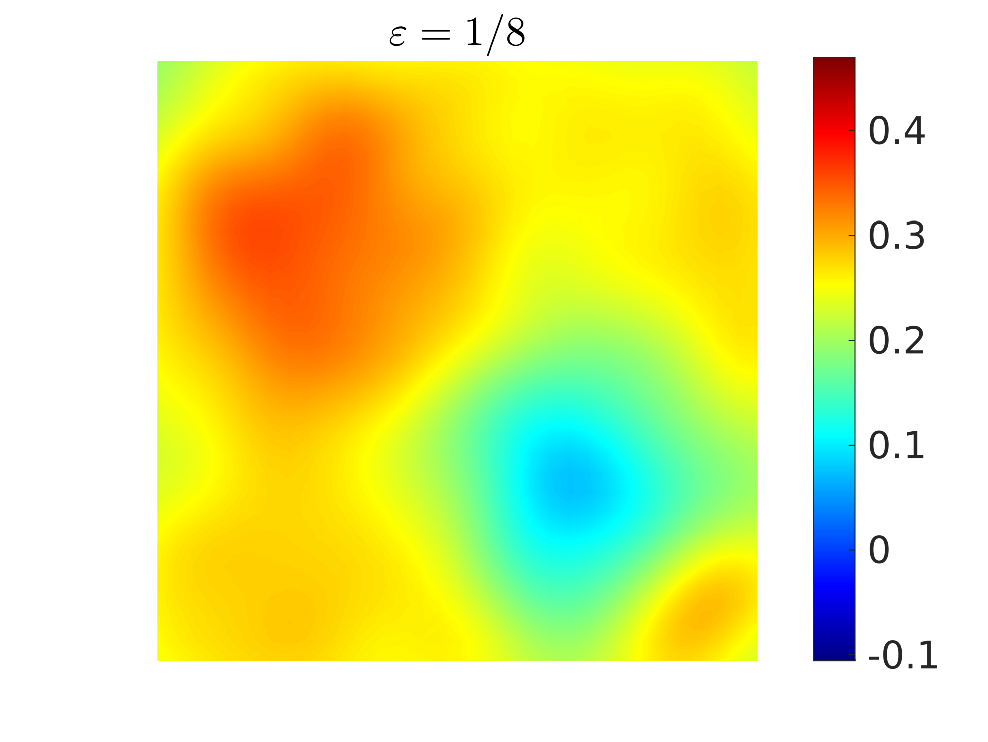
\includegraphics[width = 0.45\textwidth]{Images/ensemble_500_e8_model_error}
\end{figure}
\end{frame}

\begin{frame}
\frametitle{Online modelling error estimation}
\begin{figure}[t]
\centering
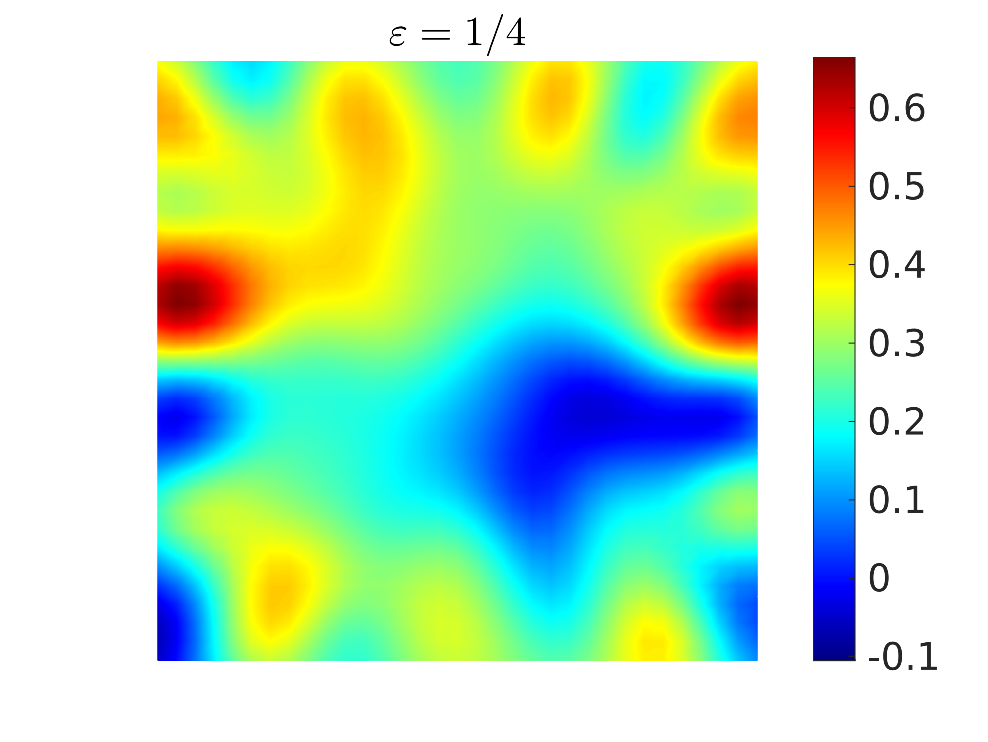
\includegraphics[width = 0.45\textwidth]{Images/ensemble_500_e4}
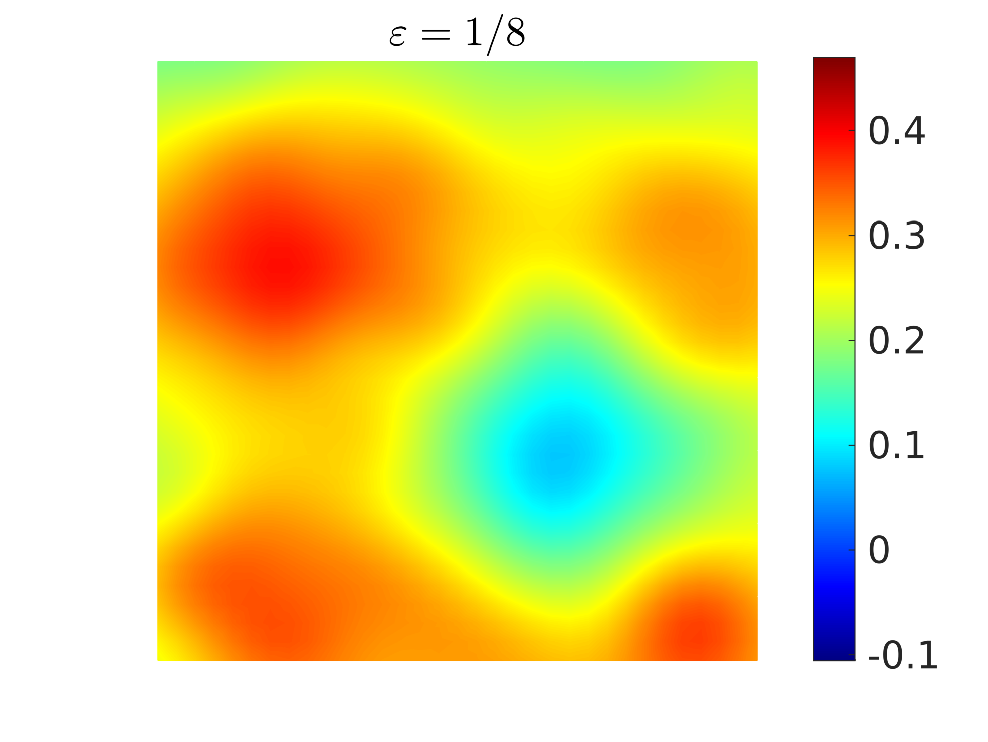
\includegraphics[width = 0.45\textwidth]{Images/ensemble_500_e8}
\\
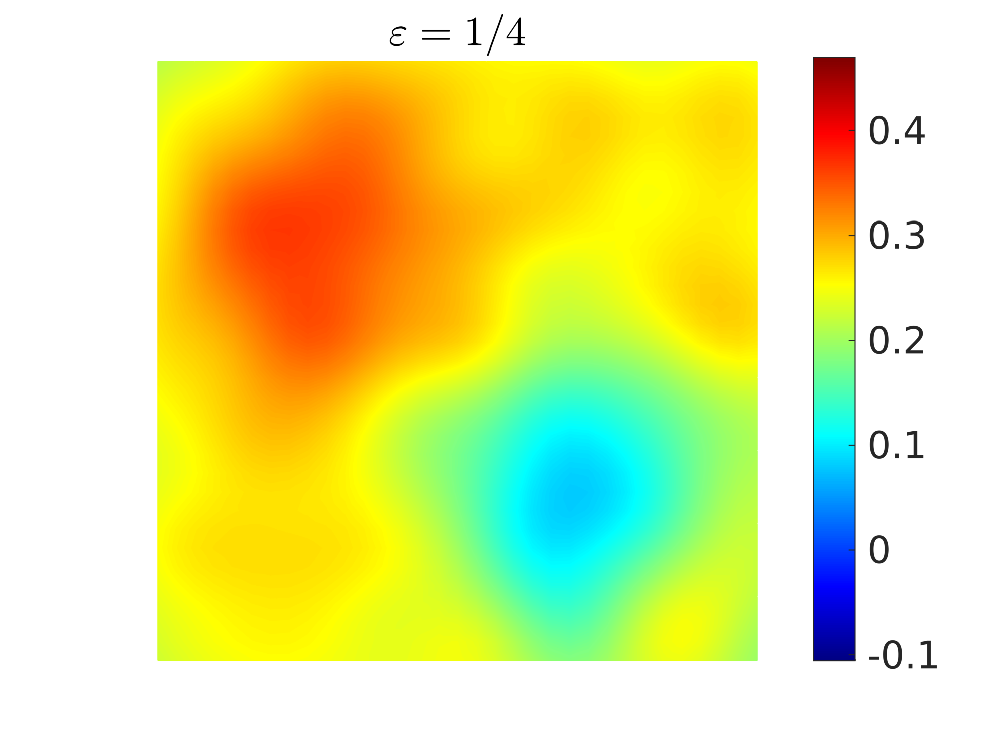
\includegraphics[width = 0.45\textwidth]{Images/ensemble_500_e4_model_error_Levels}
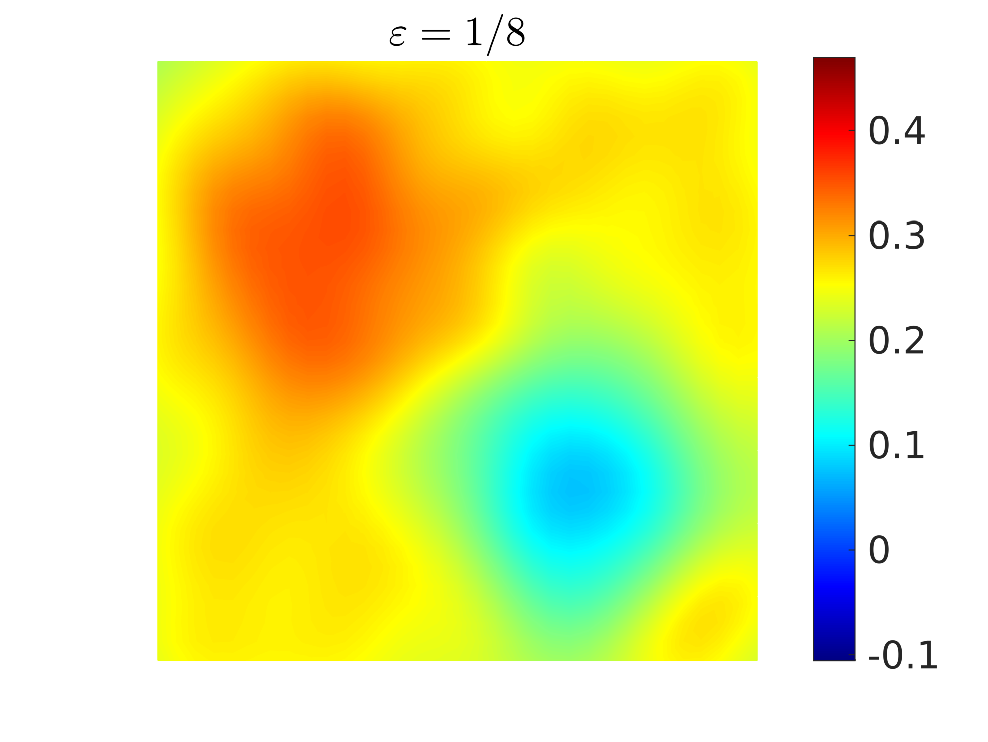
\includegraphics[width = 0.45\textwidth]{Images/ensemble_500_e8_model_error_Levels}
\end{figure}
\end{frame}

\begin{frame}
\frametitle{Conclusions}
\begin{itemize}
\setlength\itemsep{2em}
\item The ensemble Kalman filter can be used for multiscale inverse problems
\item The multiscale forward operator can be replaced by the homogenized one, taking into account the modelling error when $\varepsilon$ is big
\item The ensemble Kalman filter is easily parallelizable to reduce the computational time
\end{itemize}
\end{frame}

\begin{frame}
\frametitle{References}
\small
\bibliographystyle{apalike}
\bibliography{Bibliography}
\end{frame}

\end{document}